\section{Theoretical Analysis}
\label{sec:analysis}

\subsection{Question 1: Node Analysis}
This preliminary analysis of the circuit is the basis of the rest of the work and to do this we used the nodal method in the same way as used in T1. We have the equations: (the nomenclature for all nodes and branches is present in figure 1).\par
\emph{Node 0 (ground):}
\begin{equation}
    \frac{1}{R_1}(V_2-V_1) + \frac{1}{R_4}(V_5-0)- I_d  = 0
\end{equation}\par

\emph{Node 2:}
\begin{equation}
    \frac{1}{R_1}(V_1-V_2) + \frac{1}{R_2}(V_3-V_2) + \frac{1}{R_3}(V_5-V_2) = 0
\end{equation}\par

\emph{Node 3:}
\begin{equation}
    \frac{1}{R_2}(V_2-V_3) + I_b  = 0
\end{equation}\par

\emph{Node 5:}
\begin{equation}
    \frac{1}{R_3}(V_2-V_5) + \frac{1}{R_5}(V_6-V_5) + \frac{1}{R_4}(0-V_5) - I_d = 0
\end{equation}\par

\emph{Node 6:}
\begin{equation}
    \frac{1}{R_5}(V_5-V_6) - I_b - I_c = 0
\end{equation}\par

\emph{Node 7:}
\begin{equation}
    \frac{1}{R_6}(V_7-0) + I_d  = 0
\end{equation}\par

\emph{Node 8:}
\begin{equation}
    \frac{1}{R_7}(V_7-V_8) - I_d + I_c = 0
\end{equation}\par

\emph{Additional equation:}
\begin{equation}
     V_5 - V_8 - K_dI_d = 0
\end{equation}\par

\emph{Additional equation:}
\begin{equation}
     V_2 - V_5 - \frac{I_b}{K_b} = 0
\end{equation}\par

And the results are shown in the following table:

\begin{center}
  \begin{tabular}{ | c | c | }
    \hline    
    {\bf Name} & {\bf Value [A or V]} \\ \hline
    $V_1$ & 5.025226e+00 \\ \hline 
$V_2$ & 4.724476e+00 \\ \hline 
$V_3$ & 4.104661e+00 \\ \hline 
$V_5$ & 4.765766e+00 \\ \hline 
$V_6$ & 5.702373e+00 \\ \hline 
$V_7$ & -1.847813e+00 \\ \hline 
$V_8$ & -2.790649e+00 \\ \hline 
$I_1$ & -2.870701e-04 \\ \hline 
$I_2$ & -3.006765e-04 \\ \hline 
$I_3$ & 1.360640e-05 \\ \hline 
$I_4$ & 1.190255e-03 \\ \hline 
$I_5$ & 3.006765e-04 \\ \hline 
$I_6$ & 9.031846e-04 \\ \hline 
$I_7$ & 9.031846e-04 \\ \hline 
$I_s$ & -2.870701e-04 \\ \hline 
$I_d$ & 9.031846e-04 \\ \hline 
$I_b$ & -3.006765e-04 \\ \hline 
$I_c$ & -2.168404e-19 \\ 

    \hline
  \end{tabular}
\end{center}
All the variables preceded by I are currents and are expressed in Ampere, the other variables, preceeded by V are voltages and are expressed in Volt.



\subsection{Question 2: Equivalent Resistance ($R_{eq}$)}
The resolution of this question was based on the suggestion presented. Firstly, we set $V_s =0$ and replaced the capacitor by a voltage source $V_x = V_6 - V_8$ and ran the nodal analysis in order to obtain the current $I_x$ witch is the current supplied by $V_x$.\par
Then, with the equation: 
\begin{equation}
     R_{eq} = \frac{V_x}{I_x}
\end{equation}\par
We obtain the Equivalent resistance. \par 
The time constant $\tau$ is calculated by doing $\tau=R_{eq}C$\par
 Since the capacitor was replaced by a Voltage source witch terminals have the same difference of potential as $V_6 - V_8$ in Question 1, this is a known variable that corresponds to $V_x$ ($V_{eq}$). $I_x$ can also be obtainned by running the nodal method with $V_s = 0$. We needed to do this because there is no faster way to calculate the Equivalent Resistance in a circuit where there are resistances in paralell, in series and a capacitor. Basically, the procedure was based on \emph{Thévenin} theorem to obtain $V_{eq}$. By doing this, we have $V_{eq}=R_{eq}I_x$, where $R_{eq}$ is the only unknown variable. \par

The results:

\begin{center}
  \begin{tabular}{ | c | c | }
    \hline    
    {\bf Name} & {\bf Value [A or V]} \\ \hline
    $V_x$ & 8.493021e+00 \\ \hline 
$V_1$ & 0.000000e+00 \\ \hline 
$V_2$ & 0.000000e+00 \\ \hline 
$V_3$ & -0.000000e+00 \\ \hline 
$V_5$ & 0.000000e+00 \\ \hline 
$V_6$ & 8.493021e+00 \\ \hline 
$V_7$ & 0.000000e+00 \\ \hline 
$V_8$ & 0.000000e+00 \\ \hline 
$I_1$ & 0.000000e+00 \\ \hline 
$I_2$ & 0.000000e+00 \\ \hline 
$I_3$ & 0.000000e+00 \\ \hline 
$I_4$ & 0.000000e+00 \\ \hline 
$I_5$ & 2.726493e-03 \\ \hline 
$I_6$ & -0.000000e+00 \\ \hline 
$I_7$ & -0.000000e+00 \\ \hline 
$I_s$ & 0.000000e+00 \\ \hline 
$I_d$ & -0.000000e+00 \\ \hline 
$I_b$ & 0.000000e+00 \\ \hline 
$I_x$ & 2.726493e-03 \\ \hline 
$Req (kOhm)$ & 3.114999e+00 \\ \hline 
$tau (ms)$ & 3.145605e+00 \\ 

    \hline
  \end{tabular}
\end{center}


\subsection{Question 3: Natural solution $v_{6t}(t)$}
The natural solution $v_{6t}(t)$ can be obtained in the interval $[0,20]ms$, by doing: \par
\begin{equation}
     V_6(t) = V_{6n}(t) + V_{6f}(t)
\end{equation}\par
Where:\par
\begin{equation}
     V_{6n}(t) = {A}e^{\frac{-t}{\tau}}
\end{equation}\par
And $v_{6f}(t=0s)$ because $v_s(t=0s)=0$\par
Then:
\begin{equation}
     V_6(0) = V_x(0) + V_8(0)
\end{equation}\par
So ($v_8(t=0s)=0$):
\begin{equation}
     V_6(0) = V_x(0) 
\end{equation}\par
Finally, we get the natural solution:
\begin{equation}
     V_x =  {A}e^{\frac{-t}{\tau}}
\end{equation}\par

By doing this, the plot obtained is the one shown below:

\begin{figure}[H] \centering
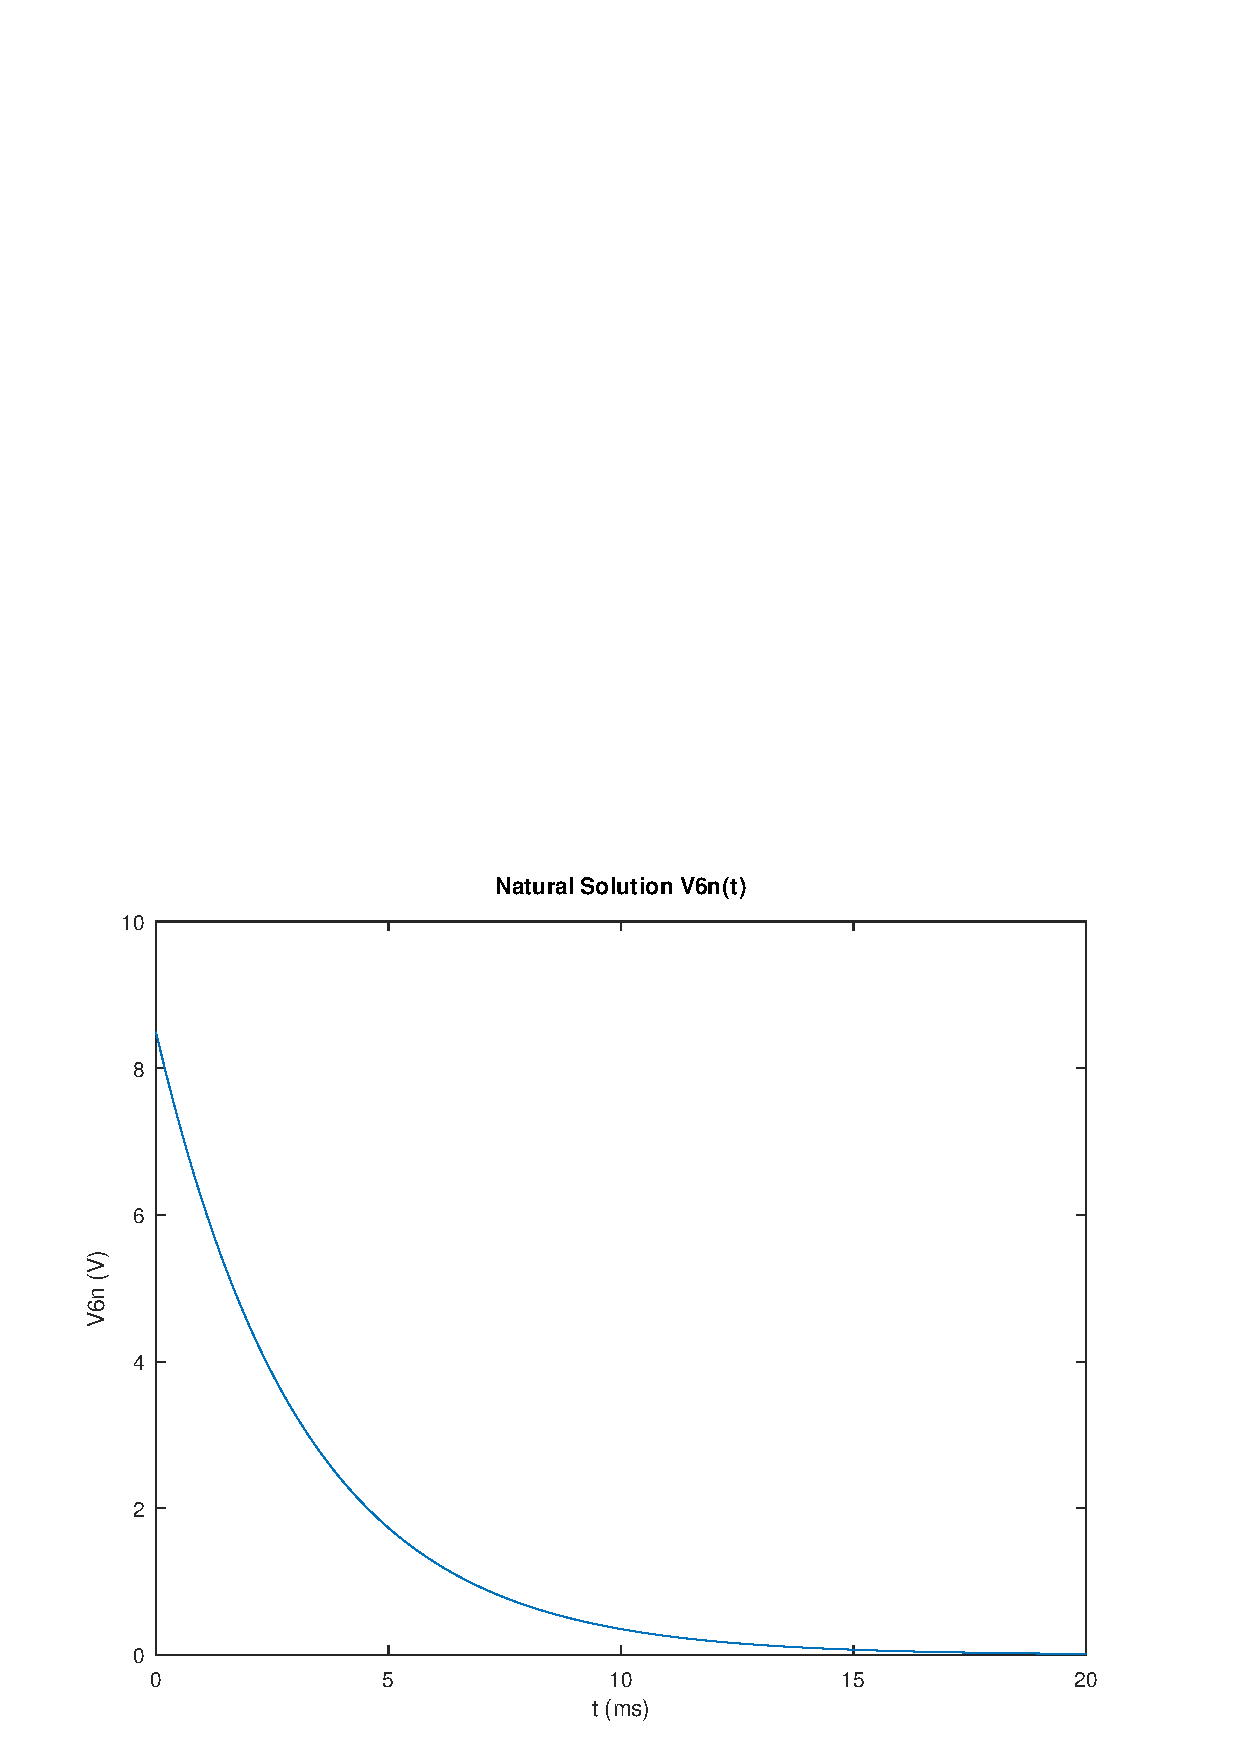
\includegraphics[width=0.7\linewidth]{../mat/alinea3.pdf}
\caption{Natural solution $v_{6t}(t)$}
\label{fig:plot3}
\end{figure}


\subsection{Question 4: Forced solution $v_{6f}(t)$ (f=1Khz)}
In this question, we have used a phasor voltage source $V_s = 1$, since $\phi = 0$, we get:
\begin{equation}
     v_s = sen(2\pi ft) => v_s = -(sen(\phi_s) + icos(\phi_s))
\end{equation}\par
So, $v_s=-i$.
\begin{equation}
     Z_c = \frac{1}{j\omega c}
\end{equation}\par
Where $\omega= 2\pi f$ and $f= 1000Hz$.\par

Then, replacing C with  impedance $Z_c$ and running the nodal analysis to determine the phasor voltages in all nodes we have the following results:\par

\begin{center}
  \begin{tabular}{ | c | c | }
    \hline    
    {\bf Name} & {\bf Value [V]} \\ \hline
    $V_1$ & 6.123234e-17 \\ \hline 
$V_2$ & 5.756770e-17 \\ \hline 
$V_3$ & 5.001526e-17 \\ \hline 
$V_5$ & 5.807082e-17 \\ \hline 
$V_6$ & 8.493021e+00 \\ \hline 
$V_7$ & -2.251559e-17 \\ \hline 
$V_8$ & -3.400403e-17 \\ 

    \hline
  \end{tabular}
\end{center}

We have calculated the module of $V_6$ with "abs" Octave's function. Then, the phase is calculated in the expression:
\begin{equation}
     phase_6 = 0 + arctan({2\pi f}{R_{eq}}{C})
\end{equation}\par

Where $R_{eq}$ and $C$ are the equivalent resistance and the Capacitor's capacitance, respectively.

And, finnaly, the forced solution is given by the expression:
\begin{equation}
     V_{6f}= V_6cos({2\pi f}{t} - phase_6)
\end{equation}\par
and the following plot:\par

\begin{figure}[H] \centering
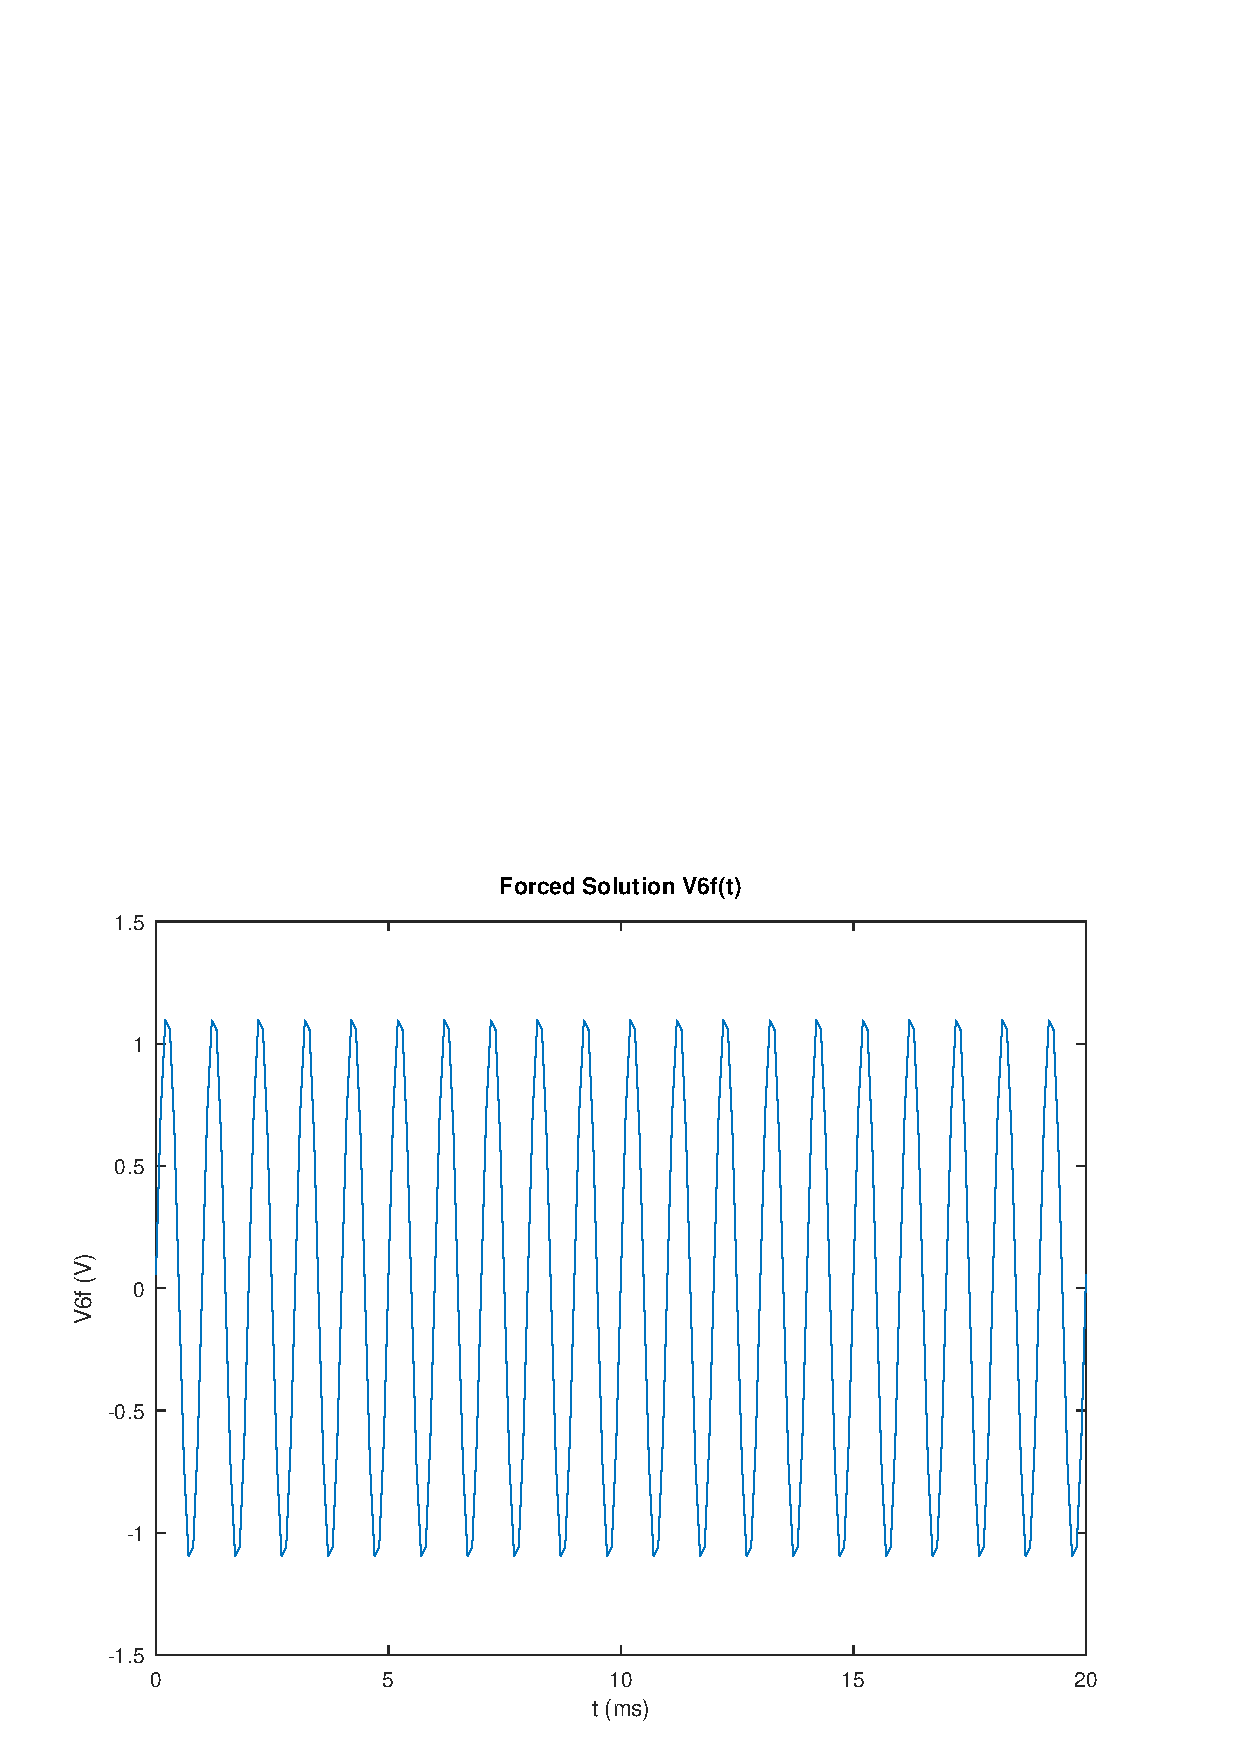
\includegraphics[width=0.7\linewidth]{../mat/alinea4.pdf}
\caption{Forced solution $v_{6t}(t)$}
\label{fig:plot4}
\end{figure}

where $V_6$ is the module value, calculated in the previous expression.



\subsection{Question 5: Final solution $v_{6}(t)$ }
The final total solution is given by:
\begin{equation}
     V_6(t) = V_{6n}(t) + V_{6f}(t)
\end{equation}\par
Considering the time period of $[0 ; 20]ms$: \par $v_s = sin(2\pi ft)$ and $v_6(t)= v_{6n}(t) + v_{6f}(t)$
Considering the time period of $[-5,0]ms$ (In this period of time there is no variation of $v_s$ and so, $v_6$ is also constant, as seen before):\par $v_s = V_s (initial value)$ and $v_6(t) =V_6$.\par
The results ($v_6(t) - blue, v_6 (t) - red$):
\begin{figure}[H] \centering
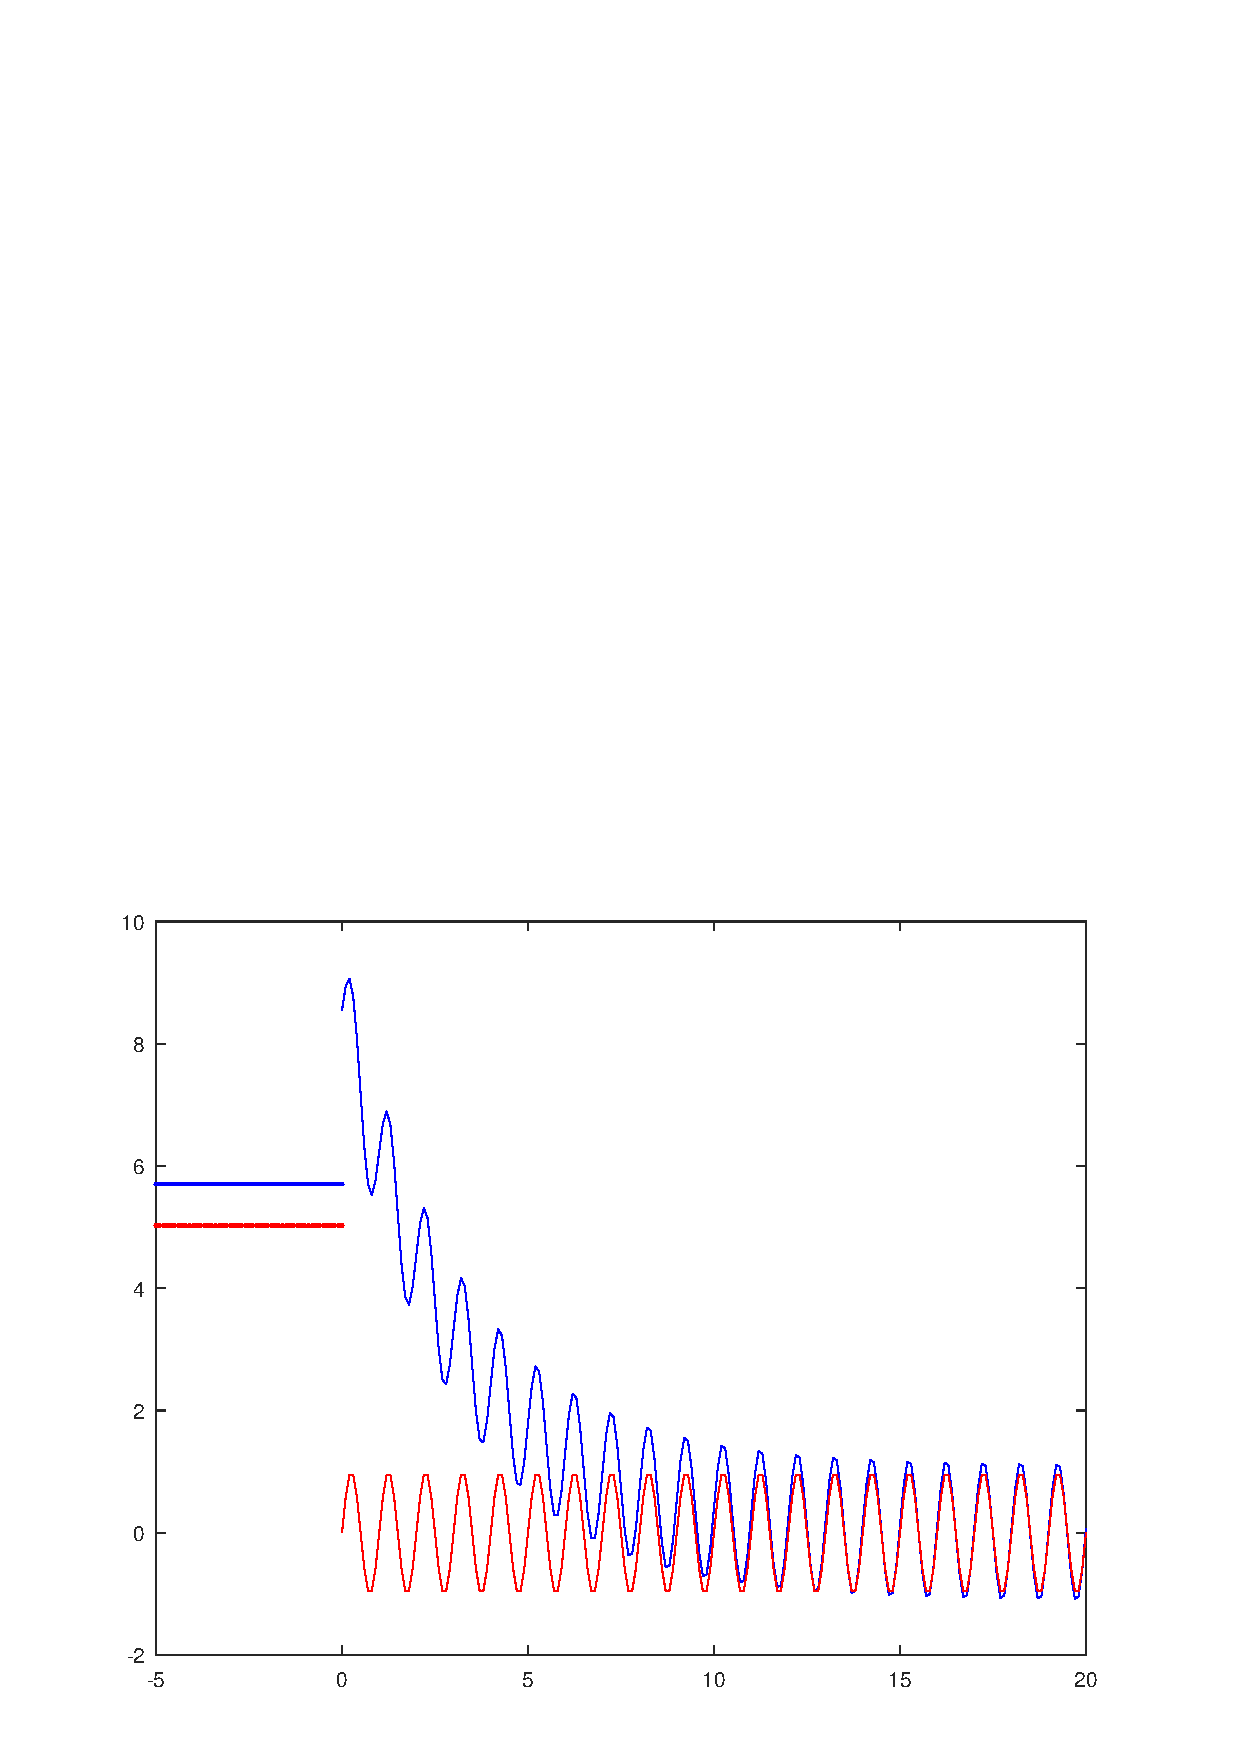
\includegraphics[width=0.7\linewidth]{../mat/alinea5.pdf}
\caption{Final solution $v_{6}(t)$}
\label{fig:plot5}
\end{figure}

\subsection{Question 6: Frequency response}
The main focus of this procedure was to determine the frequency response $v_6(f)$, $v_c(f)$ and $v_s(f)$ for a frequency range of 0.1Hz to 1Mhz (using logarithmic scale for f). \par
As mention before, the impedance expression is:
\begin{equation}
     Z_c = \frac{1}{j\omega c}
\end{equation}\par
Then, we ran the nodal analysis (like in question 4) for each value of frequency determining the phaser voltage in each node, which allowed us to determine the $v_6(f)$, $v_c(f) = v_6(f) - v_8(f)$ and $v_s(f)$ values. As seen before, the phasor voltage $v_s$ value is independet from he frequency and so, it is constant ($v_s = -i$). \par
We have used the magnitude values in dB and phase in degrees, in order to represent the results:\par
\begin{equation}
     magnitude (dB) = 20log_{10}(abs(x))
\end{equation}\par
And,
\begin{equation}
     phase (degrees) = \frac{180}{\pi}angle(x)
\end{equation}\par
where x is the phasor voltage.\par
The $v_s$ is the \textcolor{blue}{blue} line, $v_c$ \textcolor{green}{green} and the $v_6$ the \textcolor{red}{red} one.\par
The results are shown in the following plots:

\begin{figure}[H] \centering
\includegraphics[width=0.7\linewidth]{../mat/alinea61.pdf}
\caption{Magnitude of phasor voltages ($dB$)}
\label{fig:plot6}
\end{figure}

\begin{figure}[H] \centering
\includegraphics[width=0.7\linewidth]{../mat/alinea62.pdf}
\caption{Phase of phasor voltages (degrees)}
\label{fig:plot7}
\end{figure}





